\section{Principal Component Analysis (\textit{PCA})}

\begin{frame}[allowframebreaks]{Постановка задачи}
    Дан неразмеченный датасет $X = \{\boldsymbol{x}_i\}_{i=1}^N$, где $\boldsymbol{x}_i \in \mathbb{R}^D$.
    Предполагаем центрированность данных: $\mathbb{E}[\boldsymbol{x}_i] = 0$.

    Матрица ковариации данных:
    \begin{equation*}
        \boldsymbol{\Sigma} = \frac{1}{N}\sum_{i=1}^N\boldsymbol{x}_i\boldsymbol{x}_i^T.
    \end{equation*}

    Переход в новое пространство меньшей размерности (сжатие):
    \begin{equation*}
        \boldsymbol{z}_i = \mathbf{B}^T\boldsymbol{x}_i \in \mathbb{R}^M, \quad M<D,
    \end{equation*}

    \framebreak

    Базис $\mathbf{B} = [\boldsymbol{b}_1, \ldots, \boldsymbol{b}_M] \in \mathbb{R}^{D \times M}$ удовлетворяет:
    \begin{equation*}
        \boldsymbol{b}_i^T \boldsymbol{b}_j = \delta_{ij} = \begin{cases}
            0, & i\neq j, \\
            1, & i=j.
        \end{cases}
    \end{equation*}

    Восстановление данных:
    \begin{equation*}
        \tilde{\boldsymbol{x}}_i = \mathbf{B}\boldsymbol{z}_i.
    \end{equation*}
\end{frame}

\begin{frame}{Пример: 2D \(\to\) 1D}
    Исходный вектор: $\boldsymbol{x}_i \in \mathbb{R}^2$, $\boldsymbol{x}_i = \begin{bmatrix} 5 \\ \frac{1}{100} \end{bmatrix}$.
    Выбираем базис $\mathbf{B} = \begin{bmatrix} 1 \\ 0 \end{bmatrix}$.

    \textbf{Шаги:}
    \begin{itemize}
        \item Координаты в новом базисе: $\boldsymbol{z}_i = \mathbf{B}^T\boldsymbol{x}_i = 5.$
        \item Восстановленный вектор: $\tilde{\boldsymbol{x}}_i = \mathbf{B}\boldsymbol{z}_i = \begin{bmatrix} 5 \\ 0 \end{bmatrix}.$
    \end{itemize}

    \begin{columns}
        \column{0.5\textwidth}
        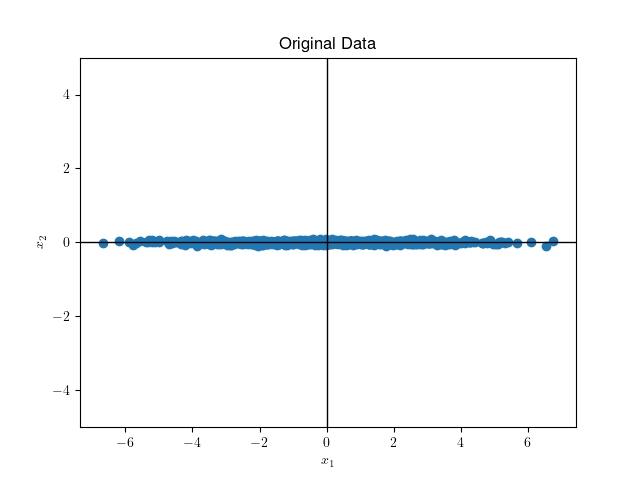
\includegraphics[width=0.8\textwidth]{../resources/pca/simple_example.png}

        \column{0.5\textwidth}
        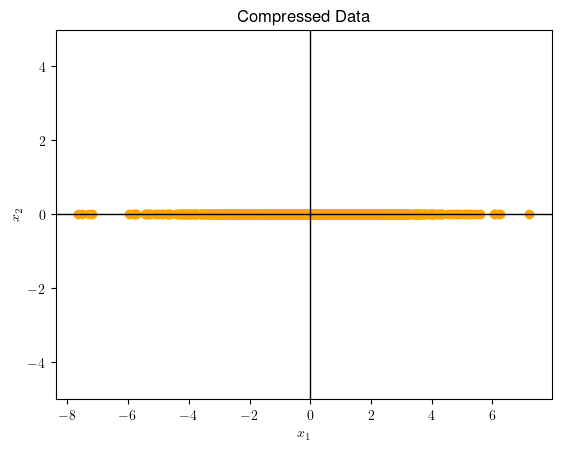
\includegraphics[width=0.8\textwidth]{../resources/pca/simple_example_comp.png}
    \end{columns}
\end{frame}

\begin{frame}[allowframebreaks]{Нахождение направления максимальной дисперсии}
    \textbf{Цель:} Найти направление $\boldsymbol{b}_1$, вдоль которого дисперсия данных максимальна.

    Дисперсия вдоль первой координаты в новом пространстве:
    \begin{align*}
        V_1 := \mathbb{D}[z_1] & = \frac{1}{N}\sum_{i=1}^Nz_{1i}^2 = \frac{1}{N}\sum_{i=1}^N(\boldsymbol{b}_1^T\boldsymbol{x}_i)^2  = \frac{1}{N}\sum_{i=1}^N(\boldsymbol{b}_1^Tx_ix_i^T\boldsymbol{b}_1) \\
                               & = \boldsymbol{b}_1^T\left(\frac{1}{N}\sum_{i=1}^Nx_ix_i^T\right)\boldsymbol{b}_1 = \boldsymbol{b}_1^T\boldsymbol{\Sigma}\boldsymbol{b}_1.
    \end{align*}

    \framebreak

    Задача условной оптимизации:
    $$
        \max_{\boldsymbol{b}_1} \boldsymbol{b}_1^T \boldsymbol{\Sigma} \boldsymbol{b}_1, \quad\text{s.t.} \: \boldsymbol{b}_1^T \boldsymbol{b}_1 = 1.
    $$

    Функция Лагранжа: \(\mathcal{L}(\boldsymbol{b}_1, \lambda) = \boldsymbol{b}_1^T \boldsymbol{\Sigma} \boldsymbol{b}_1 - \lambda(\boldsymbol{b}_1^T \boldsymbol{b}_1 - 1)\).

    Частные производные по $\boldsymbol{b}_1$ и $\lambda$:

    \begin{align*}
        \frac{\partial\mathcal{L}}{\partial\boldsymbol{b}_1} & = 2\boldsymbol{\Sigma}\boldsymbol{b}_1 - 2\lambda_1\boldsymbol{b}_1 = 0, \\
        \frac{\partial\mathcal{L}}{\partial\lambda_1}        & = -\boldsymbol{b}_1^T\boldsymbol{b}_1 + 1 = 0.
    \end{align*}
\end{frame}

\begin{frame}{Собственные векторы и значения}
    \textbf{Получаем:}
    \begin{align*}
        \boldsymbol{\Sigma} \boldsymbol{b}_1 & = \lambda_1 \boldsymbol{b}_1, \\
        V_1                                  & = \lambda_1.
    \end{align*}

    Теперь можем переписать дисперсию $V_1$ как:

    $$
        V_1 = \boldsymbol{b}_1^T\boldsymbol{\Sigma}\boldsymbol{b}_1 = \lambda_1\boldsymbol{b}_1^T\boldsymbol{b}_1 = \lambda_1.
    $$

    \textbf{Интерпретация:}
    \begin{itemize}
        \item $\boldsymbol{b}_1$: первое направление главной компоненты.
        \item $\lambda_1$: дисперсия вдоль направления $\boldsymbol{b}_1$.
    \end{itemize}
\end{frame}

\begin{frame}[allowframebreaks]{Остальные компоненты}
    \textbf{Для $m$-й компоненты:}
    \begin{align*}
         & \max_{\boldsymbol{b}_m} \boldsymbol{b}_m^T \boldsymbol{\Sigma} \boldsymbol{b}_m,                                    \\
         & \text{s.t. } \boldsymbol{b}_m^T \boldsymbol{b}_m = 1, \quad \boldsymbol{b}_m^T \boldsymbol{b}_i = 0, \forall i < m.
    \end{align*}

    Функция Лагранжа: \(
    \mathcal{L}(\boldsymbol{b}_m, \lambda_m, \boldsymbol{\mu}) = \boldsymbol{b}_m^T\boldsymbol{\Sigma}\boldsymbol{b}_m - \lambda_m(\boldsymbol{b}_m^T\boldsymbol{b}_m - 1) - \sum_{i=1}^{m-1}\mu_i\boldsymbol{b}_m^T\boldsymbol{b}_i.
    \)

    \begin{align*}
        \frac{\partial\mathcal{L}}{\partial\boldsymbol{b}_m} & = 2\boldsymbol{\Sigma}\boldsymbol{b}_m - 2\lambda_m\boldsymbol{b}_m - \sum_{i=1}^{m-1}\mu_i\boldsymbol{b}_i = 0, \\
        \frac{\partial\mathcal{L}}{\partial\lambda_m}        & = -\boldsymbol{b}_m^T\boldsymbol{b}_m + 1 = 0,\quad
        \frac{\partial\mathcal{L}}{\partial\mu_i} = -\boldsymbol{b}_m^T\boldsymbol{b}_i = 0,\:\forall i<m.
    \end{align*}

    Домножим первое уравнение на $\boldsymbol{b}_j^T,\:j<m$ слева:

    $$
        2\boldsymbol{b}_j^T\boldsymbol{\Sigma}\boldsymbol{b}_m - 2\lambda_m\boldsymbol{b}_j^T\boldsymbol{b}_m - \sum_{i=1}^{m-1}\mu_i\boldsymbol{b}_j^T\boldsymbol{b}_i = 0,
    $$

    поскольку $\boldsymbol{b}_j^T\boldsymbol{b}_i = \delta_{ji}$:

    $$
        2\boldsymbol{b}_j^T\boldsymbol{\Sigma}\boldsymbol{b}_m - \mu_j = 0.
    $$

    $\boldsymbol{\Sigma}$ симметрична, поэтому $\boldsymbol{b}_j^T\boldsymbol{\Sigma}\boldsymbol{b}_m = \left\langle (\boldsymbol{b}_j^T\boldsymbol{\Sigma})^T, \boldsymbol{b}_m \right\rangle = \left\langle \boldsymbol{\Sigma}\boldsymbol{b}_j, \boldsymbol{b}_m \right\rangle = \left\langle \lambda_j\boldsymbol{b}_j, \boldsymbol{b}_m \right\rangle = \lambda_j \left\langle \boldsymbol{b}_j, \boldsymbol{b}_m \right\rangle = 0$.

    Тогда $\mu_j = 0.$ и, аналогично, $\forall j<m \:\: \mu_j=0$

    \framebreak

    Таким образом:

    $$
        \boldsymbol{\Sigma}\boldsymbol{b}_m = \lambda_m\boldsymbol{b}_m,
    $$

    Вновь, $\boldsymbol{b}_m$ - собственный вектор матрицы ковариации $\boldsymbol{\Sigma}$, а $\lambda_m$ - собственное значение.

    \textbf{Общая дисперсия:} $\sum_{i=1}^N\lambda_i$. \\
    \textbf{Объясненная дисперсия} первых $m$ главных компонент: $\sum_{i=1}^m\lambda_i$. \\
    \textbf{Доля объясненной дисперсии:} $\frac{\sum_{i=1}^m\lambda_i}{\sum_{i=1}^N\lambda_i}$.
\end{frame}

\begin{frame}{Практические аспекты реализации}
    \textbf{Формулы:}
    \begin{align*}
        \boldsymbol{Z}         & = \mathbf{B}^T \boldsymbol{X},                \\
        \tilde{\boldsymbol{X}} & = \mathbf{B} \boldsymbol{Z},                  \\
        \boldsymbol{\Sigma}    & = \frac{1}{N}\boldsymbol{X} \boldsymbol{X}^T.
    \end{align*}

    \textbf{Примечание:} строки \(\boldsymbol{X}\) — признаки, столбцы — объекты.
\end{frame}

\begin{frame}{Практика}
    \begin{figure}
        \centering
        
\includegraphics[width=.3\textwidth]{../resources/overall/Jupyter_logo.png}
    \end{figure}
\end{frame}
